\documentclass[12pt]{article}

\usepackage[utf8]{inputenc}
\usepackage[spanish]{babel}
\usepackage[vmargin=2.5cm,hmargin=2.5cm]{geometry}
\usepackage{enumerate}
\usepackage{algpseudocode}
\usepackage{graphics,graphicx,float} %para incluir imágenes y colocarlas
\usepackage{spverbatim}

\title{\vspace{5cm}
Práctica 2: Planificación de caminos en Robótica}

\author{ Elena María Gómez Ríos }


\begin{document}


\maketitle
\newpage

\section{Resumen}
En esta práctica vamos a realizar una planificación de rutas para un robot móvil con el simulador Stage. Para la planificación de rutas se va a implementar el algoritmo A* para la búsqueda del mejor camino hasta un punto objetivo elegido. Para la implementación del algoritmo A* se ha partido de la implementación proporcionada por los profesores de la búsqueda en anchura.\\

El algoritmo A* utilizará una heurística basada en el coste de los posibles caminos desde el origen del robot móvil hasta el punto objetivo, favoreciendo el camino cuyo coste sea mínimo. Además se contempla la seguridad del robot por el mapa eliminando aquellos caminos que consideremos no seguros, ya sea porque no puede pasar o hay un obstáculo cerca.\\

En las siguientes secciones se explicará con más detalle la implementación usada del algoritmo A*. Y por último llevaremos a cabo una experimentación del algoritmo que hemos implementado detallando tiempo, nodos expandidos y longitud del camino encontrado de varias ejecuciones sobre el mapa ``willow-garage''. 


\newpage


\section{Descripción de la solución planteada}

El problema de la búsqueda del mejor camino hasta un punto objetivo se ha resuelto con la implementación del algoritmo A* con una heurística basada en la distancia.

\subsection{Algoritmo A*}
El algoritmo A* genera un valor para cada nodo mediante la función $f(n)$, la cual está compuesta por la suma de una valor heurístico $h(n)$ y el coste real conocido del camino recorrido para llegar a dicho nodo $g(n)$, es decir, $f(n) = g(n)+h(n)$.\\

Siendo $g(n)$ la distancia recorrida desde el nodo origen hasta el nodo anterior al explorado más la distancia del nodo anterior al nodo explorado en este camino. Y para $h(n)$ tomamos la distancia en línea recta entre el nodo explorado y el nodo objetivo.


He realizado una serie de pasos para encontrar el mejor camino, basándome en la implementación de la búsqueda en anchura proporcionada:
\begin{enumerate}
\item Disponemos de una lista para los nodos abiertos y otra para los nodos cerrados. La lista de nodos abiertos se ordena por el valor de la función $f(n)$ para obtener los mejores nodos primero, mediante la función \texttt{compareFCost} la cual compara la $f(n)$ de los nodos.
\item En la implementación inicial no se miraba al generar un nuevo vecino aquellos nodos que estuviesen en la lista de cerrados o abiertos. Para mejorar esto ahora si miramos estos nodos, comprobando si tienen mejor coste $g(n)$ que el anterior y de ser así cambiándolo por el nuevo de forma recursiva. Igualmente si el nodo está en abiertos y tiene un mejor coste lo modificamos cambiando su enlace al mejor padre.
\item Al añadir los vecinos a la lista de nodos abiertos tenemos en cuenta si un nodo es seguro o no antes de añadirlo. Esto lo hago mediante el método \texttt{cercaObjeto} el cuál nos indica si hay un objeto demasiado cerca del nodo, en concreto a una distancia de tres casillas del nodo, y por tanto sería un camino no seguro y así poder ignorar dicho nodo.
\end{enumerate}



\section{Experimentación}
Para la experimentación he realizado tres ejecuciones distintas en las cuales muestro dos capturas de cada una de las ejecuciones en las que se puede apreciar los nodos abiertos de color verde y el camino elegido con una línea de color rojo.

\begin{figure}[H] 
	\centering
	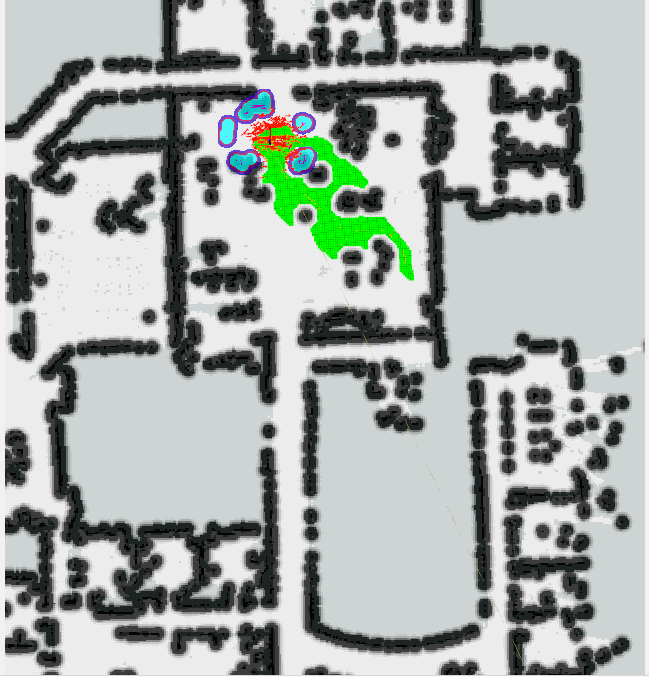
\includegraphics[width=8cm]{img/exp_1_1.png}
	\caption{Experimentación 1 - Nodos Abiertos}
\end{figure}


\begin{figure}[H] 
	\centering
	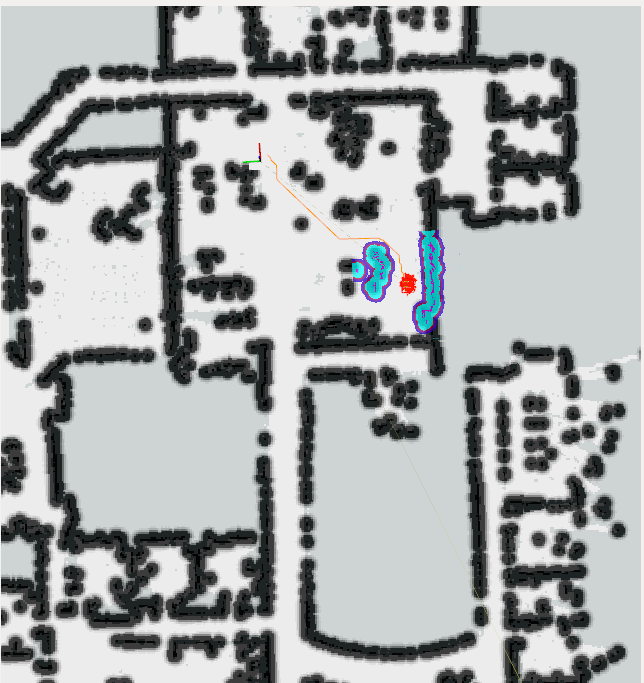
\includegraphics[width=8cm]{img/exp_1_2.png}
	\caption{Experimentación 1 - Camino}
\end{figure}


\begin{figure}[H] 
	\centering
	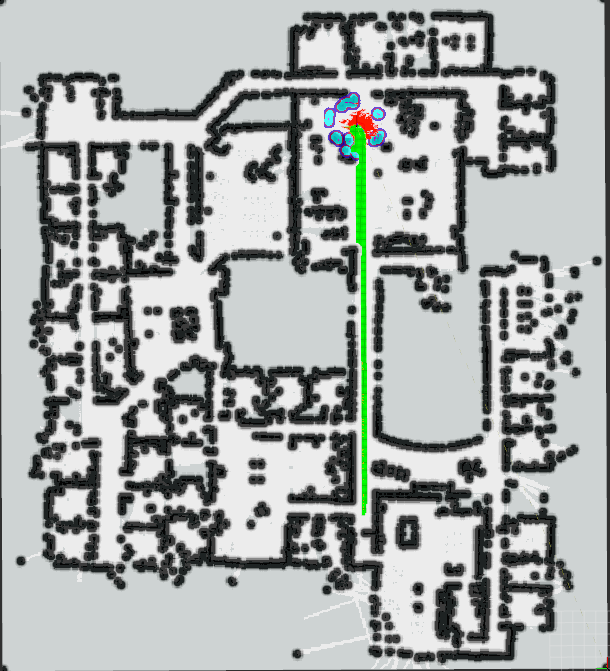
\includegraphics[width=8cm]{img/exp_2_1.png}
	\caption{Experimentación 2 - Nodos Abiertos}
\end{figure}


\begin{figure}[H] 
	\centering
	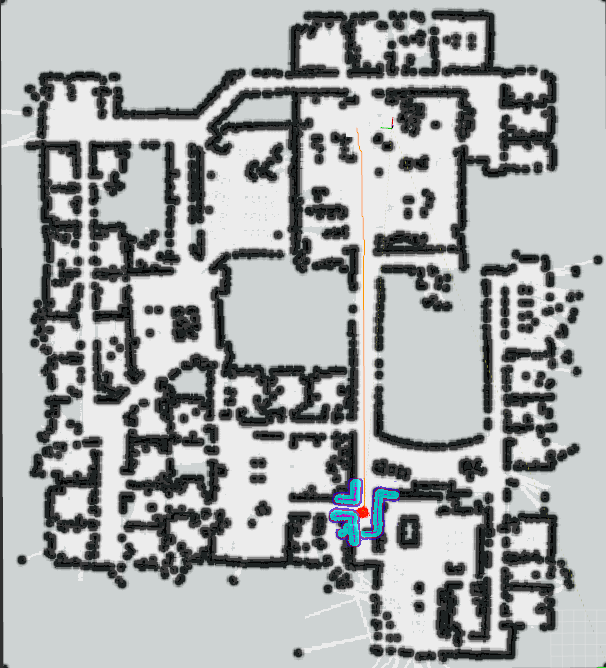
\includegraphics[width=8cm]{img/exp_2_2.png}
	\caption{Experimentación 2 - Camino}
\end{figure}

\begin{figure}[H] 
	\centering
	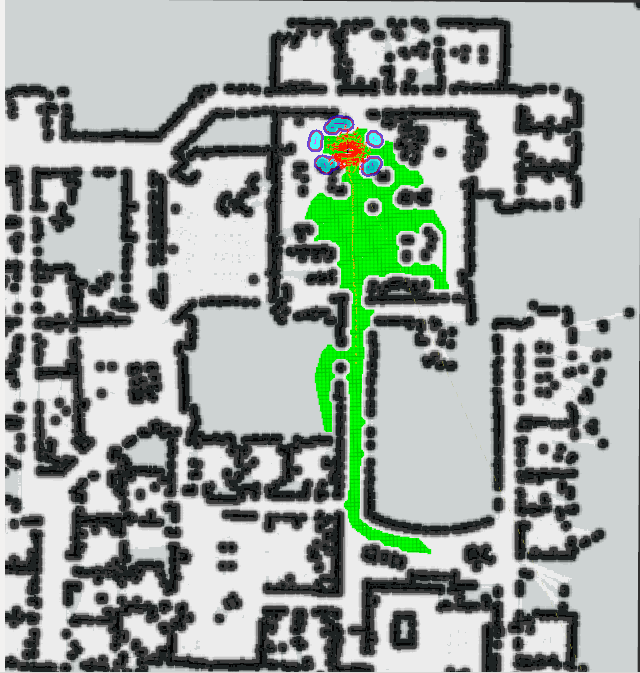
\includegraphics[width=8cm]{img/exp_3_1.png}
	\caption{Experimentación 3 - Nodos Abiertos}
\end{figure}


\begin{figure}[H] 
	\centering
	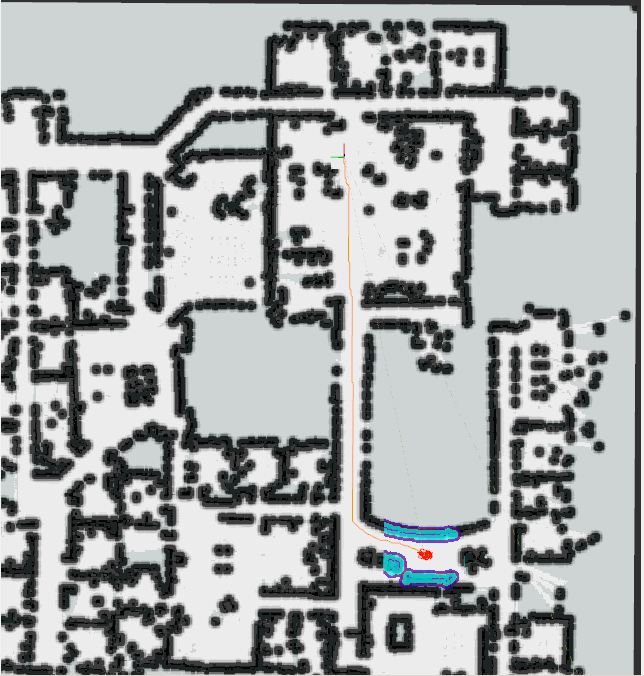
\includegraphics[width=8cm]{img/exp_3_2.png}
	\caption{Experimentación 3 - Camino}
\end{figure}

\begin{table}[H]
\centering
\caption{Tabla de resultados de las experimentaciones}
\label{my-label}
\begin{tabular}{|c|c|c|c|}
\hline
                                                                                              & Experimentación 1 & Experimentación 2 & Experimentación 3 \\ \hline
Tiempo de ejecución (segundos)                                                                & 6                 & 8                 & 15                \\ \hline
Nodos expandidos                                                                              & 1775              & 1377              & 6972              \\ \hline
\begin{tabular}[c]{@{}c@{}}Longitud del camino encontrado\\             en nodos\end{tabular} & 99                & 330               & 324               \\ \hline
\begin{tabular}[c]{@{}c@{}}Longitud del camino encontrado\\ en metros\end{tabular}            & 12.236751         & 33.431365         & 33.866891         \\ \hline
\end{tabular}
\end{table}


\end{document}